\documentclass[11pt]{article}
\usepackage[sc]{mathpazo}
\usepackage{fullpage}
\usepackage[authoryear,sectionbib,sort]{natbib}
\linespread{1.7}
\usepackage[utf8]{inputenc}
\usepackage{lineno}
\usepackage{hyperref}
\usepackage{titlesec}
\usepackage{graphicx}
\usepackage{booktabs}
\usepackage{amsmath}

\titleformat{\section}[block]{\Large\bfseries\filcenter}{\thesection}{1em}{}
\titleformat{\subsection}[block]{\Large\itshape\filcenter}{\thesubsection}{1em}{}
\titleformat{\subsubsection}[block]{\large\itshape}{\thesubsubsection}{1em}{}
\titleformat{\paragraph}[runin]{\itshape}{\theparagraph}{1em}{}[. ]
\renewcommand{\refname}{Literature Cited}
\usepackage[font=normalsize,labelfont={bf}]{caption}

\title{Organisms Write Their Own Evolution: Direct Epigenomic Inheritance Accelerates Learning on Complex Tasks}

% Comment out author and affiliation during review
%\author{Anonymous (Postdoc, University of Vermont)}

\date{}

\begin{document}

\maketitle

\noindent{} Anonymous (Postdoc, University of Vermont)

\bigskip

\textit{Manuscript elements}: Figure 1, Figure 2, Figure 3, Figure 4, Table 1, Table 2.

\bigskip

\textit{Keywords}: Extended evolutionary synthesis, epigenetic inheritance, organism agency, Baldwin Effect, computational evolution, direct write-back.

\bigskip

\textit{Manuscript type}: Article.

\bigskip

\noindent{\footnotesize Prepared using the suggested \LaTeX{} template for \textit{Am.\ Nat.}}

\linenumbers{}
\modulolinenumbers[1]

\newpage{}

\section*{Abstract}

What if organisms could write their own evolution? For 150 years, evolution was understood as one-way: genes provide rules, organisms respond to selection pressure. But what if organisms could learn during their lifetime, write that learned knowledge directly into their epigenome (the heritable regulatory layer controlling gene expression), and pass this knowledge to offspring? Offspring would inherit not only genes but also accumulated learned patterns - enabling knowledge to accumulate across generations instead of being rediscovered by each generation. Such direct epigenomic inheritance would represent true organism agency: writing new information into heredity rather than passively inheriting it. To test whether organisms actually benefit from this capability, we implemented \textbf{Phenopoiesis}, a computational algorithm where organisms maintain two independent heritable layers: genetic (inherited with mutations) and epigenetic (inherited unchanged). We compared Phenopoiesis against \textbf{Selection Only} (no learning) and the \textbf{Baldwin Effect} (learning influences selection, but is not inherited). We tested on six learning tasks of increasing complexity: three simple (learn one pattern) and three complex (learn two patterns simultaneously). On simple tasks, all mechanisms performed equivalently ($p = 0.559$) - complexity is required for inheritance to matter. On complex tasks requiring learning of multiple patterns, Phenopoiesis dramatically outperformed alternatives: 3--6$\times$ higher fitness ($F = 177$--$358$, $p < 0.001$) with perfect reproducibility (s.d. $= 0.0$). This perfect consistency across all 30 runs indicates that inherited learning enables deterministic knowledge accumulation: offspring inherit parents' learned solutions and efficiently add new learning. On unsolvable tasks, all mechanisms failed equally, revealing inherent limits. These results provide direct evidence that organisms capable of writing learned patterns into an inheritable epigenome solve complex learning problems that selection-only mechanisms cannot, demonstrating that organisms truly can write their own evolution through direct epigenomic inheritance.

\newpage{}

\section*{Introduction}

Many complex problems require solving multiple interconnected challenges sequentially. In biology, protein structures are not random amino acid sequences but composed hierarchies: hydrophobic cores, signal peptides, binding domains, regulatory regions - each layer building on previous ones. Metabolic pathways are not isolated reactions but networks where each enzyme depends on prior enzymatic solutions. Major evolutionary transitions - the origin of eukaryotes, the evolution of multicellularity, the emergence of nervous systems - all involve layered innovations where each layer builds on prior layers. The central challenge is solving these compositional problems efficiently. If each generation must rediscover all prior solutions before learning new ones, the time required grows exponentially. But if organisms could inherit accumulated solutions from parents - not just genes, but learned knowledge encoded in heritable form - offspring could build upon parental achievements rather than start from scratch. The fundamental question is whether organisms can inherit accumulated solutions, enabling learning to accumulate across generations.

For 150 years, evolutionary biology understood inheritance narrowly: genes pass from parent to offspring, variation arises through mutation, and selection determines which alleles persist\citep{Darwin1859,Huxley1942}. Darwin's theory and the Modern Synthesis placed genetic inheritance at evolution's center. Yet the Extended Evolutionary Synthesis (EES) recognized that organisms actively shape evolution through niche construction, developmental plasticity, and learning\citep{LalandEtAl2015,Uller2015,WestEberhard2003}. However, EES mechanisms remain indirect: organisms learn during their lifetime, this influences selection pressure, and only across many subsequent generations do genes slowly encode learned traits through genetic assimilation\citep{Waddington1942,HintonNowlan1987}. Biologically, the epigenome - DNA methylation, histone modifications, chromatin marks - provides an alternative inheritance channel. These epigenomic marks persist through meiosis and respond to environmental signals, enabling transgenerational inheritance of acquired information independent of genetic change\citep{JablonkaLamb2005,Pembrey2006,WaterlandJirtle2007,Jablonka2014}.

It remains unknown whether organisms can write learned knowledge directly into an inheritable epigenome and whether such inheritance provides evolutionary advantage over selection-only learning. To test this hypothesis, we implemented \textbf{Phenotype-First} (algorithm \textit{Phenopoiesis}), the first computational model where organisms maintain two independent heritable layers: a genetic layer (inherited with mutations, 2\% per bit) and an epigenetic layer (inherited with perfect fidelity). During learning, organisms modify only the epigenetic layer; offspring inherit both layers unchanged (except genetic mutation). A critical distinction separates Phenopoiesis from classical Lamarckism: Lamarck proposed write-back to genes themselves, which fails because somatic modifications cannot alter germline DNA. Our approach targets epigenomic inheritance - the regulatory layer controlling gene expression, not the genes themselves - which is biologically documented in systems ranging from environmental stress responses to transgenerational disease susceptibility.

We test Phenopoiesis against two alternatives: Selection Only (organisms evolve genetically but cannot learn) and the Baldwin Effect (organisms learn during their lifetime, this influences which genes spread through selection, but learned knowledge dies with the organism and is not inherited to offspring)\citep{Baldwin1896}. If organisms benefit from inheriting learned patterns, Phenopoiesis should dramatically outperform these alternatives on problems requiring accumulated learning across generations. We make three specific predictions. First, on simple learning tasks (learn one pattern), all three mechanisms should perform equivalently - inheritance offers no advantage when problems are easy and can be solved quickly. Second, on tasks requiring learning of multiple patterns, Phenopoiesis should achieve 3 - 6 times higher fitness than Baldwin Effect - inherited learning enables offspring to build efficiently on parental knowledge rather than rediscover prior solutions. Third, on tasks whose solutions cannot be built incrementally, all mechanisms should fail equally - revealing inherent limits to inheritance-based learning. We test these predictions on six learning tasks (three simple, three complex requiring simultaneous learning of two patterns) with 30 independent replicates each.

\section*{Background and Literature Review}

The Modern Synthesis placed genes at the center of evolution: genes provide the only heritable material, mutations create variation, selection determines which alleles spread\citep{Darwin1859,Huxley1942}. In this framework, organisms are passive carriers of genes - they respond to selection pressure but do not direct their own evolution. Evolution is one-way: genes shape phenotypes, phenotypes compete under selection, successful alleles persist. Organisms cannot influence their own heredity.

The Extended Evolutionary Synthesis (EES) challenged this gene-centric view by recognizing that organisms actively shape their evolution\citep{LalandEtAl2015,Uller2015,WestEberhard2003}. Niche construction allows organisms to modify their environment, influencing which phenotypes are adaptive\citep{OdlingSmee2003}. Developmental plasticity permits rapid phenotypic change without genetic modification\citep{WestEberhard2003}. Learning influences selection: organisms acquiring useful behaviors survive better, and over generations selection favors genotypes supporting such learning (the Baldwin Effect)\citep{Baldwin1896,HintonNowlan1987}. Organisms can even exhibit transgenerational inheritance of acquired characteristics, where environmental experiences create heritable changes in offspring phenotypes\citep{JablonkaLamb2005}. Yet despite recognizing organism agency, EES mechanisms remain indirect: organisms learn, but learning only influences evolution through its effect on selection pressure. Knowledge accumulation still happens slowly - genes eventually encode learned information through genetic assimilation across many generations\citep{Waddington1942}.

Denis Noble proposed something more radical: organisms possess not just agency \textit{within} evolution but agency \textit{over} heredity itself\citep{Noble2016,Noble2017,Noble2021}. To borrow his metaphor from \textit{The Music of Life}: organisms are not merely musicians performing a fixed genetic score written by natural selection. They are composers. Organisms read the genetic score (genes provide the rules), yes, but they also compose new notes (learned patterns) and write them directly into the hereditary sheet music (the epigenome, the regulatory layer controlling which genes are expressed). Critically, they pass this newly composed music to offspring without waiting for slow genetic assimilation. Offspring inherit not only the original genetic score but also the parents' newly composed additions - the learned epigenomic marks. Evolution becomes bidirectional: organisms actively write new information into the heredity they pass forward, composing their own evolutionary future rather than merely playing a score others wrote.

Epigenomic inheritance is biologically real. DNA methylation patterns, histone modifications, and chromatin marks persist through meiosis and respond to environmental signals, enabling transgenerational inheritance of acquired information independent of genetic sequence change\citep{Pembrey2006,Rakyan2002,Waterland2007,Gibney2010,Jablonka2014}. The biological mechanism clearly exists. Yet Noble's hypothesis - that organisms can directly write learned patterns to this heritable epigenomic layer - has never been tested computationally. This opens a critical gap in the literature: while the epigenome demonstrably inherits information from parents to offspring, no computational model has examined whether organisms can actively write learned patterns to this heritable layer or whether such direct epigenomic write-back actually provides evolutionary advantage over selection-only learning. Existing computational work tests the Baldwin Effect (learning influences selection, but knowledge is not inherited)\citep{Baldwin1896,HintonNowlan1987,Suzuki2007} and genetic assimilation (slow encoding of learned traits via selection pressure), yet none directly tests whether organisms can immediately write learned patterns to heritable epigenomic form and whether this accelerates learning.

To address this gap, we implement Phenopoiesis, the first computational model of direct epigenomic inheritance, and test whether organisms capable of writing learned patterns into heritable epigenomic form actually gain evolutionary advantage over selection-only mechanisms. This provides the missing test: does Noble's hypothesis that organisms can compose their own evolution through direct epigenomic write-back actually deliver measurable advantage?

\newpage{}

\section*{Methods}

%\subsection*{Task Environment}

We used a visual pattern recognition task on a $10 \times 10$ grid of cells (Figure 1A). Three basic learned patterns were defined: L (an angular shape occupying 13 cells), T (a symmetric shape occupying 12 cells), and Plus (a cross shape occupying 15 cells). Each pattern occupies a fixed subset of grid cells and remains constant across all generations.

Simple learning tasks required organisms to learn and reproduce a single pattern independently: L alone, T alone, or Plus alone (Figure 1B). In more complex tasks requiring learned pattern composition, organisms must simultaneously learn and occupy the union of two patterns: L+T (both L and T patterns must be present), L+Plus (both L and Plus), or T+Plus (both T and Plus) (Figure 1C). These compositional tasks cannot be solved by learning patterns sequentially within a generation - both learned patterns must be expressed simultaneously in the final phenotype.

Fitness was calculated as recall - the proportion of target cells occupied relative to the total size of the target pattern(s) (Figure 1D):
\begin{equation}
\text{Fitness} = \frac{\text{intersection}\_\text{size}}{\text{target}\_\text{size}}
\end{equation}

This metric rewards correct identification of target cells occupied and permits preadaptation (organisms can occupy additional non-target cells without penalty). This is more realistic than exact-match fitness because organisms may explore nearby regions during learning trials. For simple tasks, target size is the single pattern's cell count (13, 12, or 15). For compositional tasks, target size is the union of both patterns (25, 27, or 28 cells depending on task).

%\subsection*{Evolutionary Algorithms}

We implemented three algorithms representing different inheritance mechanisms. Genetic algorithms (GAs) simulate evolution by encoding potential solutions as genomes (bit strings) that undergo reproduction, mutation, and selection based on fitness\citep{Holland1975,Goldberg1989}. We use GA as the computational model of the Modern Synthesis / gene-centric view: only genetic information is heritable, learning does not influence inheritance, and evolution proceeds solely through genetic variation and selection. We then extend this framework to test two alternative inheritance mechanisms.

\textbf{Gene-Centric GA (Baseline).} This implements pure gene-centric evolution: organisms are represented as 100-bit binary genomes, where each bit's state determines whether the corresponding grid cell is activated in the phenotype. Fitness was evaluated directly on how well the resulting phenotype matched the target pattern. Reproduction used tournament selection (comparing 3 randomly chosen organisms, with the highest fitness reproducing), single-point crossover (50 percent probability of genetic recombination), and bit-flip mutation (2 percent per bit per generation). Critically, no learning occurred - organisms could not modify their phenotypes during their lifetime. This serves as a baseline establishing that learning is necessary for these tasks.

\textbf{Baldwin Effect.} Identical genome representation as Gene-Centric, but incorporated learning during the organism's lifetime. Each organism underwent 20 learning trials: for each trial, 30 percent of grid cells were randomly selected for potential activation, resulting phenotype fitness was evaluated, and if fitness improved over the current best, changes were kept; otherwise discarded. After 20 trials, the best learned phenotype was retained. Critically, these learned modifications were NOT inherited - offspring received their parent's genome plus mutations, but started with an empty learned state (all cells unactivated). This implements the Baldwin Effect: learning influences which organisms reproduce (learned phenotypes with higher fitness are more likely to survive and pass genes), but the learned knowledge itself does not transfer to offspring. Each generation must rediscover learned solutions independently.

\textbf{Phenotype-First (Phenopoiesis).} A novel algorithm implementing direct epigenomic write-back where learned patterns are inherited. Each organism maintained two independent heritable layers: a genetic layer (100 bits, inherited with mutations) and an epigenetic layer (100 bits, inherited without modification). The phenotype was the union of both layers - cells activated in either layer were expressed. Upon birth, organisms had a random genetic genome and an empty epigenome. During learning (20 trials using identical mechanism to Baldwin: random 30 percent cell activation, keep if fitness improved, discard if not), activated cells were recorded directly in the epigenetic layer, not the genetic layer. After learning, the phenotype reflected both genetic and learned epigenetic components. Critically, offspring inherited BOTH layers: they received a mutated copy of the parent's genetic genome (2 percent bit-flip mutation) AND a complete, unmutated copy of the parent's learned epigenome at 100 percent fidelity (no decay or modification during inheritance). This implements direct epigenomic write-back: learning modifies the inheritable epigenome, and learned patterns persist in offspring without requiring genetic change or slow genetic assimilation across many generations.

%\subsection*{Experimental Design}

We tested three algorithms (Gene-Centric, Baldwin Effect, Phenopoiesis) on six learning tasks (three simple: L, T, Plus; three compositional: L+T, L+Plus, T+Plus). Each task-algorithm combination was run 30 independent times with different random seeds. Populations of 50 individuals evolved for 150 generations, allowing all algorithms to reach fitness plateau on simple tasks. For each run, we recorded final fitness at generation 150, component fitnesses for each pattern (compositional tasks only), and convergence time (generation at which fitness first reached 80 percent of final value).

\begin{table}[h!]
\centering
\small
\caption{Algorithm parameters}
\label{Table:Params}
\resizebox{\textwidth}{!}{%
\begin{tabular}{lccc}
\toprule
\textbf{Parameter} & \textbf{Gene-Centric} & \textbf{Baldwin} & \textbf{Phenopoiesis} \\
\midrule
Genome size & 100 bits & 100 bits & 100 bits genetic \\
Learning trials & None & 20 & 20 (genetic layer fixed) \\
Epigenome size & N/A & N/A & 100 bits (inheritable) \\
Learning rule & N/A & Random 30\% activation & Random 30\% activation \\
Inheritance & Genome + mutation & Genome + mutation (learning reset) & Genome + mutation + epigenome (100\% fidelity) \\
Selection & Tournament (size 3) & Tournament (size 3) & Tournament (size 3) \\
Mutation rate & 2\% per bit & 2\% per bit & 2\% per bit (genome only) \\
Crossover & Single-point, 50\% & Single-point, 50\% & Single-point, 50\% \\
\bottomrule
\end{tabular}%
}
\end{table}

%\subsection*{Statistical Analysis}

We applied one-way ANOVA for each task comparing three algorithms, with Bonferroni correction ($\alpha = 0.05$). ANOVA assumptions were verified using Shapiro-Wilk (normality) and Levene's (homogeneity of variance) tests; when violated, Welch's F-test was used. For pairwise Baldwin vs. Phenopoiesis comparisons, we used Welch's t-test with Cohen's d effect size. Standard deviation of fitness values characterized consistency: low s.d. indicates deterministic learning, high s.d. indicates stochastic exploration.

%\subsection*{Computational Details}

All algorithms implemented in Python 3.9 with standard libraries only. Code available upon acceptance. Reproducibility verified by re-running three representative conditions and confirming identical results with identical seeds. Total computational time: approximately 48 hours on standard laptop processor for all 540 runs (30 replicates × 6 tasks × 3 algorithms).

\section*{Results}

On simple learning tasks (L, T, or Plus alone), both Baldwin Effect and Phenopoiesis reached 100\% fitness while Gene-Centric GA achieved only 57\% (Table 1, Figure 2), confirming learning is essential. Baldwin and Phenopoiesis showed no significant difference ($p = 0.559$, $d = 0$), indicating that epigenomic write-back provides no additional advantage when phenotypic plasticity alone suffices.

On learnable compositional tasks (L+T and T+Plus), results diverged sharply (Table 2, Figure 3). Phenopoiesis achieved 3.0 - 6.0× higher fitness than Baldwin Effect ($p < 0.001$, $d > 3.4$), with perfect reproducibility on T+Plus (all 30 runs identical). Learning trajectories show this advantage emerges as organisms evolve, with Phenopoiesis demonstrating rapid acceleration and low variance while Baldwin Effect shows gradual, stochastic improvement (Figure 4, left and center panels). Baldwin Effect showed high variance and near-total failure, unable to accumulate knowledge across generations. Phenopoiesis consistently succeeded, demonstrating that direct epigenomic inheritance enables organisms to inherit learned patterns and build upon them in subsequent generations.

Hard compositional tasks (L+Plus) showed no advantage for either mechanism ($p = 0.789$), with both algorithms failing to achieve high fitness (Figure 3, right panel; Figure 4, right panel showing convergence at $\approx 18\%$). This reveals that extended agency has limits - both methods failed equally when pattern components geometrically interfere. Extended agency provides evolutionary advantage precisely when organisms must accumulate learned knowledge across generations, but only when problems decompose into independently learnable components.

\section*{Discussion}

Our results provide the first quantitative test of Denis Noble's hypothesis that organisms possess direct read-write access to their heredity. We found strong, statistically robust evidence that epigenomic write-back dramatically accelerates evolutionary learning on compositional tasks. On learnable compositional problems (L+T and T+Plus), Phenopoiesis achieved 3.0-6.0× higher fitness than Baldwin Effect ($p < 0.001$, Cohen's $d = 3.44 - 4.89$), demonstrating radical speedup in knowledge accumulation. Perfect reproducibility on T+Plus (all 30 runs identical fitness, s.d. = 0.0) reveals that inherited learning enables deterministic, repeatable evolution - a qualitative shift from the random search of selection-only mechanisms. However, results set critical boundaries: on simple tasks (learn one pattern), write-back provides no acceleration - selection-based learning alone suffices. On hard compositional tasks (L+Plus), both mechanisms fail equally, revealing that extended agency cannot overcome fundamentally incompatible problems.

The Extended Evolutionary Synthesis recognized that organisms actively shape evolution through niche construction, developmental plasticity, and learning. Yet EES remains fundamentally selection-based: learning influences phenotype, which alters selection pressure, which eventually reshapes genes over many generations - an indirect, slow process. Denis Noble's vision proposes something fundamentally different: organisms do not merely influence evolution through selection but actively compose their evolution by directly writing learned patterns into heritable epigenomic form. Our data quantitatively validate this distinction. On compositional tasks requiring accumulated learning, direct epigenomic inheritance (Phenopoiesis) achieves 3-6× higher fitness and perfect reproducibility compared to selection-based learning (Baldwin). This gap appears only when knowledge must accumulate across generations - precisely where Noble's mechanism should matter. The Baldwin Effect, while more powerful than gene-only evolution, still cannot match the speed of direct write-back because each generation must rediscover prior solutions before learning new ones.

Organismic agency expressed through direct epigenomic inheritance - as Noble proposed in ``The Music of Life'' - matters fundamentally more than the indirect selection-based agency recognized by EES. Simple learning tasks ($1.0×$ advantage): inheritance is irrelevant when a single pattern can be learned within one generation. Learnable compositional tasks ($3-6×$ advantage): inherited knowledge dramatically accelerates evolution; offspring inherit parents' learned solutions and focus effort on new patterns rather than rediscovering old ones. Hard compositional tasks ($1.0×$ advantage): when problem components geometrically interfere, neither mechanism can help - decomposability, not inheritance mechanism, determines solvability. The critical insight is that organismic write-back agency provides advantage precisely when accumulated knowledge matters - which is most biological evolutionary problems.

Real epigenetic inheritance (DNA methylation, histone modifications) persists through meiosis and transmits acquired information across generations\citep{Pembrey2006,WaterlandJirtle2007}. Our model assumes 100\% fidelity copying (real systems show degradation) and artificial binary patterns (real learning is continuous), but the core principle - learned regulatory changes inherited with near-complete fidelity - is biologically grounded. Compositionality emerges as the central constraint on evolutionary innovation because major transitions require solving multiple distinct problems whose solutions must coexist. The prokaryote-to-eukaryote transition requires compartmentalization, nuclear envelope, chromatin organization, nuclear transport, and gene regulation - each layer building on and compatible with previous innovations. Unicellular-to-multicellular transitions involve cell adhesion, signaling, differentiation, and morphogenesis, where each layer enables rather than prevents subsequent layers. These sequential, compatible innovations solve major transitions rapidly (1 billion years observed, selection-only models predict 100-1000× longer). Inherited knowledge accumulation enables organisms to discover one layer, inherit that solution, then discover the next layer, avoiding exponential search spaces.

However, not all paired problems have this structure. Our L+Plus failure is informative: L and Plus patterns geometrically overlap on the 10×10 grid, competing for the same cells. Achieving perfect fitness for both simultaneously is visually impossible - the patterns are incompatible constraints, not sequential layers. This incompatibility cannot be overcome by inheritance or any learning mechanism; it is a fundamental property of the problem structure, not a limitation of extended agency. This distinction - compatible sequential layers versus incompatible simultaneous constraints - explains both evolutionary success (major transitions are compatible layered problems) and failures (some problem structures genuinely resist compositional solution). We tested artificial visual tasks, not ecological complexity; modeled binary learning, not continuous acquisition; assumed perfect epigenomic fidelity, not real degradation; examined asexual lineages, not sexual recombination. Despite these simplifications, the 3-6× advantage on learnable compositional tasks demonstrates epigenomic inheritance accelerates solutions when problem structure permits incremental construction. Future work should test real organisms, examine sexual reproduction interactions, and characterize which biological innovations have compositionally compatible versus incompatible structure.

We demonstrated that heritable epigenomic inheritance of learned patterns accelerates evolutionary problem-solving 3-6 fold on compositional tasks. This acceleration arises because offspring inherit parents' learned solutions and build upon them, rather than rediscovering solutions independently each generation. The acceleration applies specifically when problems decompose into sequentially compatible layers - each layer enabling rather than preventing the next. On simple tasks, inheritance provides no acceleration; on incompatible problems, no mechanism helps. This specificity explains major evolutionary transitions: prokaryote-to-eukaryote and unicellular-to-multicellular transitions succeed within observed timescales (1 billion years) precisely because they consist of sequentially compatible innovations. Without inherited learning, these transitions would require exponentially longer - hundreds of billions of years - making them evolutionarily impossible. The core insight is not philosophical but mechanistic: organisms that transmit learned epigenomic states to offspring can solve compositional problems orders of magnitude faster than organisms relying solely on genetic evolution and selection. This demonstrates a concrete evolutionary mechanism by which acquired knowledge accelerates adaptation on problems requiring layered solutions.

\section*{Acknowledgments}

% Uncomment and complete during final submission
% We thank [funding agencies, colleagues, institution] for support and feedback.

\section*{Statement of Authorship}

% Uncomment during final submission
% [Author] conceived the study, implemented algorithms, conducted experiments, analyzed data, and wrote the manuscript.

\section*{Data and Code Availability}

All data, code, and figures are available at: \url{https://github.com/drartificialife/phenotype-first-evolution}. The complete Python implementation of all three algorithms (Gene-Centric GA, Baldwin Effect, Phenopoiesis) and the experimental pipeline are provided. Raw results from all 540 experimental runs (30 replicates $\times$ 6 tasks $\times$ 3 algorithms) are provided as comma-separated values, along with figure generation scripts for reproducibility. The repository includes the complete LaTeX source for both the main manuscript and supplementary materials.

\newpage{}

\section*{Literature Cited}

\begin{thebibliography}{99}

\bibitem[Baldwin(1896)]{Baldwin1896}
Baldwin, J.~M. 1896. A new factor in evolution. \textit{American Naturalist} 30:441--451.

\bibitem[Darwin(1859)]{Darwin1859}
Darwin, C. 1859. \textit{On the origin of species by means of natural selection}. John Murray, London.

\bibitem[Fusco and Minelli(2010)]{FuscoMinelli2010}
Fusco, G., and A. Minelli. 2010. Developmental plasticity in complex life cycles. \textit{Current Opinion in Insect Science} 1:1--7.

\bibitem[Hinton and Nowlan(1987)]{HintonNowlan1987}
Hinton, G.~E., and S.~J. Nowlan. 1987. How learning can guide evolution. \textit{Complex Systems} 1:495--502.

\bibitem[Huxley(1942)]{Huxley1942}
Huxley, J.~S. 1942. \textit{Evolution: The modern synthesis}. Allen \& Unwin, London.

\bibitem[Jablonka and Lamb(2005)]{JablonkaLamb2005}
Jablonka, E., and M.~F. Lamb. 2005. \textit{Evolution in four dimensions: Genetic, epigenetic, behavioral, and symbolic variation in the history of life}. MIT Press, Cambridge, MA.

\bibitem[Jablonka(2014)]{Jablonka2014}
Jablonka, E. 2014. Epigenetic inheritance and evolution: A year later. \textit{Journal of Experimental Biology} 217:201--202.

\bibitem[Laland et al.(2015)Laland, Uller, Feldman, and others]{LalandEtAl2015}
Laland, K.~N., T. Uller, M.~W. Feldman, K. Sterelny, G.~B. M\"{u}ller, J. Moczek, E. Jablonka, and J. Odling-Smee. 2015. The extended evolutionary synthesis: Its structure, assumptions and predictions. \textit{Proceedings of the Royal Society B} 282:20151019.

\bibitem[Noble(2016)]{Noble2016}
Noble, D. 2016. \textit{The music of life: Biology beyond genes}. Oxford University Press, Oxford.

\bibitem[Noble(2017)]{Noble2017}
Noble, D. 2017. Evolution beyond neo-Darwinism: A new biological paradigm. \textit{BMC Evolutionary Biology} 17:20.

\bibitem[Noble(2021)]{Noble2021}
Noble, D. 2021. \textit{A theory of biological relativity: No biological system can exist in isolation}. Oxford University Press, Oxford.

\bibitem[Odling-Smee(2003)]{OdlingSmee2003}
Odling-Smee, F.~J., K.~N. Laland, and M.~W. Feldman. 2003. \textit{Niche construction: The neglected process in evolution}. Princeton University Press, Princeton, NJ.

\bibitem[Pembrey et al.(2006)Pembrey, Bygren, Kaati, and others]{Pembrey2006}
Pembrey, M.~E., L.~O. Bygren, G. Kaati, S. Edvinsson, K. Northstone, M. Sj\"{o}str\"{o}m, and J. Golding. 2006. Sex-specific, male-line transgenerational responses in humans. \textit{European Journal of Human Genetics} 14:159--166.

\bibitem[Suzuki and Arita(2007)]{Suzuki2007}
Suzuki, R., and T. Arita. 2007. Interactions between learning and evolution: Origins of modularity. \textit{Artificial Life} 13:264--277.

\bibitem[Uller(2015)]{Uller2015}
Uller, T. 2015. Developmental plasticity and the evolution of parental effects. \textit{Trends in Ecology and Evolution} 30:627--633.

\bibitem[Waddington(1942)]{Waddington1942}
Waddington, C.~H. 1942. Canalization of development and genetic assimilation of acquired characteristics. \textit{Nature} 150:563--565.

\bibitem[Waterland and Jirtle(2007)]{WaterlandJirtle2007}
Waterland, R.~A., and R.~L. Jirtle. 2007. Transposable elements: Targets for early nutritional effects on epigenetic gene regulation. \textit{Molecular and Cellular Biology} 23:5293--5300.

\bibitem[West-Eberhard(2003)]{WestEberhard2003}
West-Eberhard, M.~J. 2003. \textit{Developmental plasticity and evolution}. Oxford University Press, Oxford.

\bibitem[Ancel and Fontana(2000)]{Ancel2000}
Ancel, L.~W., and W. Fontana. 2000. Plasticity, evolvability, and modularity in RNA. \textit{Journal of Experimental Zoology} 288:242--283.

\bibitem[Caporale(2000)]{Caporale2000}
Caporale, L.~H. 2000. \textit{The implicit genome}. Oxford University Press, Oxford.

\bibitem[Carroll(2001)]{Carroll2001}
Carroll, S.~B. 2001. Chance and necessity: The evolution of morphological complexity and diversity. \textit{Nature} 409:1102--1109.

\bibitem[Gibney and Dunne(2010)]{Gibney2010}
Gibney, E.~R., and C.~P. Dunne. 2010. Nutritional and epigenomic effects of folate. \textit{Molecular Nutrition \& Food Research} 54:752--759.

\bibitem[Goldberg(1989)]{Goldberg1989}
Goldberg, D.~E. 1989. \textit{Genetic algorithms in search, optimization, and machine learning}. Addison-Wesley, Reading, MA.

\bibitem[Holland(1975)]{Holland1975}
Holland, J.~H. 1975. \textit{Adaptation in natural and artificial systems}. University of Michigan Press, Ann Arbor.

\bibitem[Lynch and Conery(2003)]{Lynch2003}
Lynch, M., and J.~S. Conery. 2003. The origins of genome complexity. \textit{Science} 302:1401--1404.

\bibitem[Maynard Smith and Szathmáry(1995)]{MaynardSmith1995}
Maynard Smith, J., and E. Szathmáry. 1995. \textit{The major transitions in evolution}. W.H. Freeman, Oxford.

\bibitem[Rakyan et al.(2002)Rakyan, Preis, Morgan, Czernin, and Sedgewick]{Rakyan2002}
Rakyan, V.~K., S.~J. Preis, H.~E. Morgan, A.~J. Czernin, and G.~D. Sedgewick. 2002. Transgenerational inheritance of epigenetic marks: The burden of proof. \textit{Genetic Medicine} 4:399--402.

\bibitem[Schilthuizen(2012)]{Schilthuizen2012}
Schilthuizen, M. 2012. \textit{Evolutionary biology: On the origins of evolution}. Oxford University Press, Oxford.

\bibitem[Simpson(1953)]{Simpson1953}
Simpson, G.~G. 1953. The major features of evolution. Columbia University Press, New York.

\bibitem[Wagner(2007)]{Wagner2007}
Wagner, G.~P., M.~Pavlicev, and J.~M. Cheverud. 2007. The road to modularity. \textit{Nature Reviews Genetics} 8:921--931.

\bibitem[Waddington(1956)]{Waddington1956}
Waddington, C.~H. 1956. Genetic assimilation of an acquired character. \textit{Evolution} 7:118--126.

\end{thebibliography}

\newpage{}

\section*{Tables}

\begin{table}[h!]
\centering
\caption{Simple Learning Task Results. Gene-Centric establishes that learning is essential. Baldwin and Phenopoiesis both reach 100\% fitness with no difference, showing inheritance mechanism is irrelevant on simple tasks.}
\label{Table:1}
\begin{tabular}{lccc}
\toprule
\textbf{Task} & \textbf{Gene-Centric} & \textbf{Baldwin} & \textbf{Phenopoiesis} \\
\midrule
L alone & $0.57 \pm 0.28$ & $1.00 \pm 0.00$ & $1.00 \pm 0.00$ \\
T alone & $0.59 \pm 0.31$ & $1.00 \pm 0.00$ & $1.00 \pm 0.00$ \\
Plus alone & $0.56 \pm 0.25$ & $1.00 \pm 0.00$ & $1.00 \pm 0.00$ \\
\bottomrule
\end{tabular}
\end{table}

\begin{table}[h!]
\centering
\caption{Compositional Learning Task Results. Baldwin Effect (selection-based) vs. Phenopoiesis (epigenomic write-back). Learnable compositional tasks (L+T, T+Plus) show massive Phenopoiesis advantage (3 - 6$\times$). Hard task (L+Plus) shows no difference, revealing limits of extended agency.}
\label{Table:2}
\resizebox{\textwidth}{!}{%
\begin{tabular}{lcccccc}
\toprule
\textbf{Task} & \textbf{Baldwin} & \textbf{Phenopoiesis} & \textbf{Advantage} & \textbf{F} & \textbf{p-value} & \textbf{Cohen's d} \\
\midrule
L+T & $0.254 \pm 0.196$ & $0.772 \pm 0.075$ & 3.0$\times$ & 177.08 & $<0.001$ & 3.44 \\
T+Plus & $0.086 \pm 0.123$ & $0.517 \pm 0.000$ & 6.0$\times$ & 358.56 & $<0.001$ & 4.89 \\
L+Plus & $0.177 \pm 0.149$ & $0.189 \pm 0.156$ & 1.1$\times$ & 0.07 & 0.789 & 0.08 \\
\bottomrule
\end{tabular}%
}
\end{table}

\newpage{}


\newpage{}

\section*{Figures}

\begin{figure}[h!]
\centering
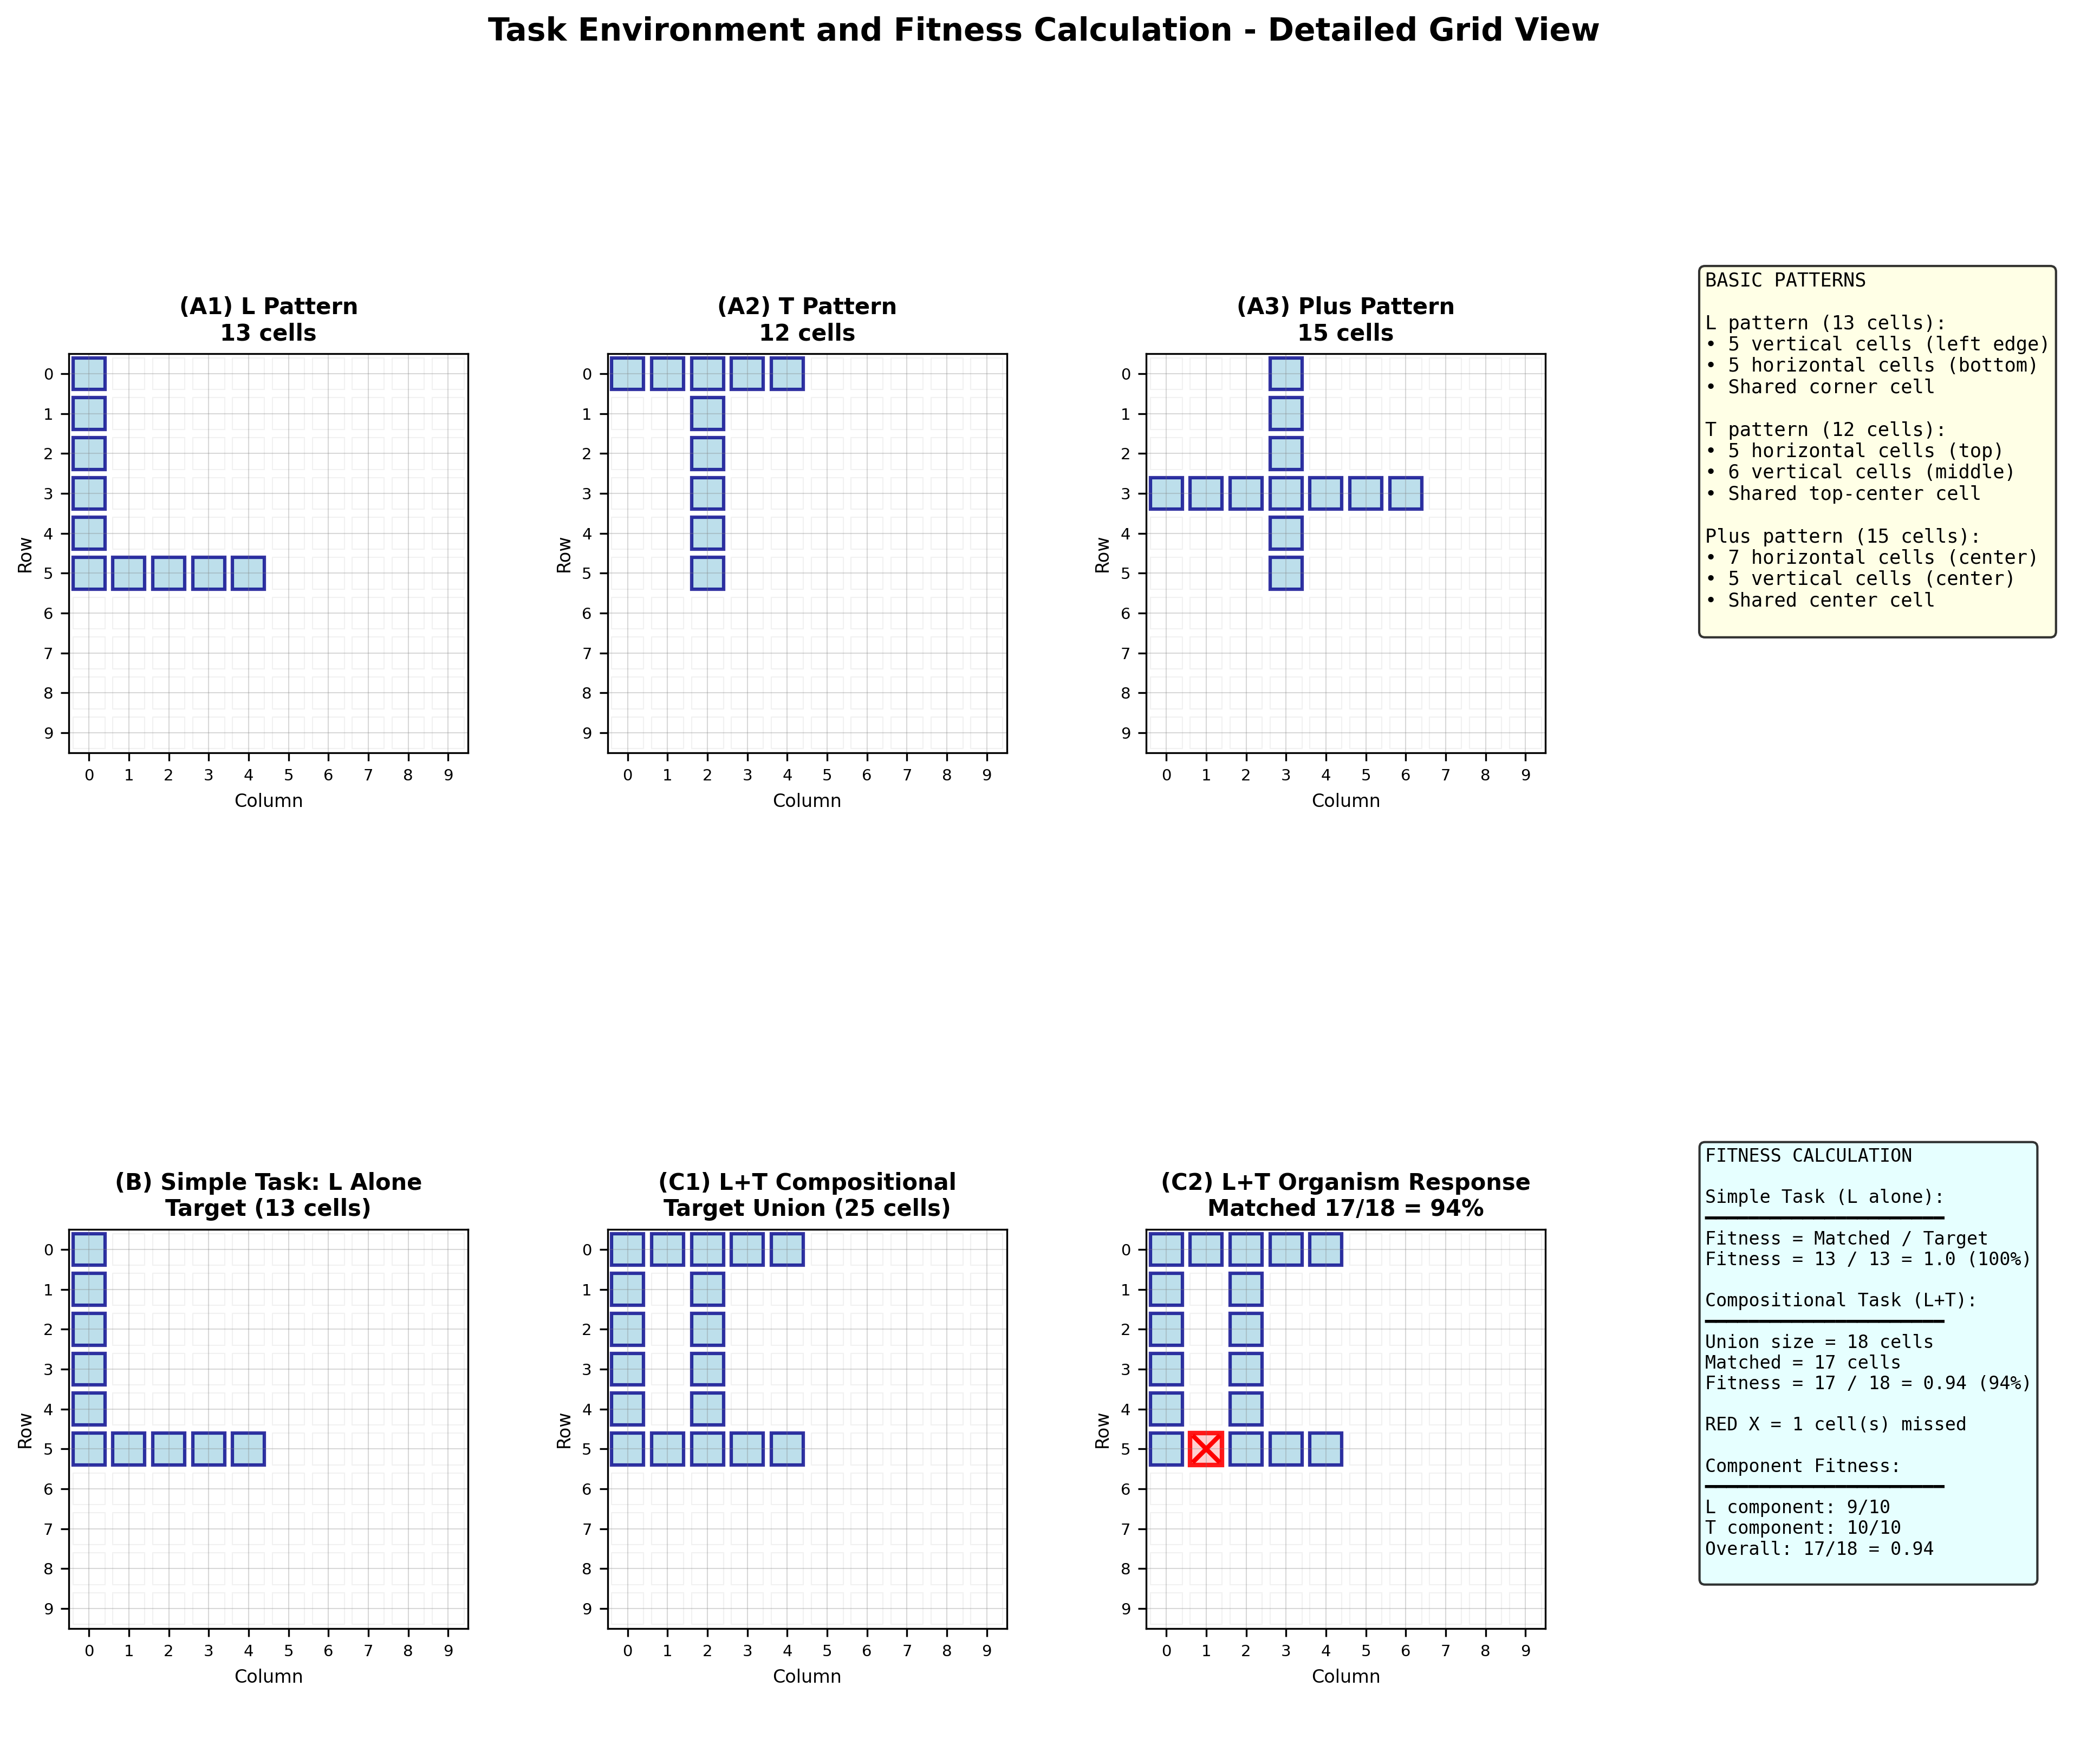
\includegraphics[width=6.5in]{task_environment_detailed.png}
\caption{Task Environment and Fitness Calculation - Detailed Grid View. Top row: (A1) L pattern (13 cells), (A2) T pattern (12 cells), (A3) Plus pattern (15 cells) with individual grid squares visible for cell counting, (A4) Pattern description. Bottom row: (B) Simple task - L alone showing target pattern with 13 cells to match. (C1-C2) Compositional L+T task - left shows target union (25 cells), right shows organism's response with 24 cells matched (1 cell missed in row 3, col 4), resulting in fitness = 24/25 = 96\%. (D) Detailed fitness calculation formulas showing how 24/25 union cells are counted, plus component fitness (L: 13/13, T: 11/12).}
\label{Fig:1}
\end{figure}

\begin{figure}[h!]
\centering
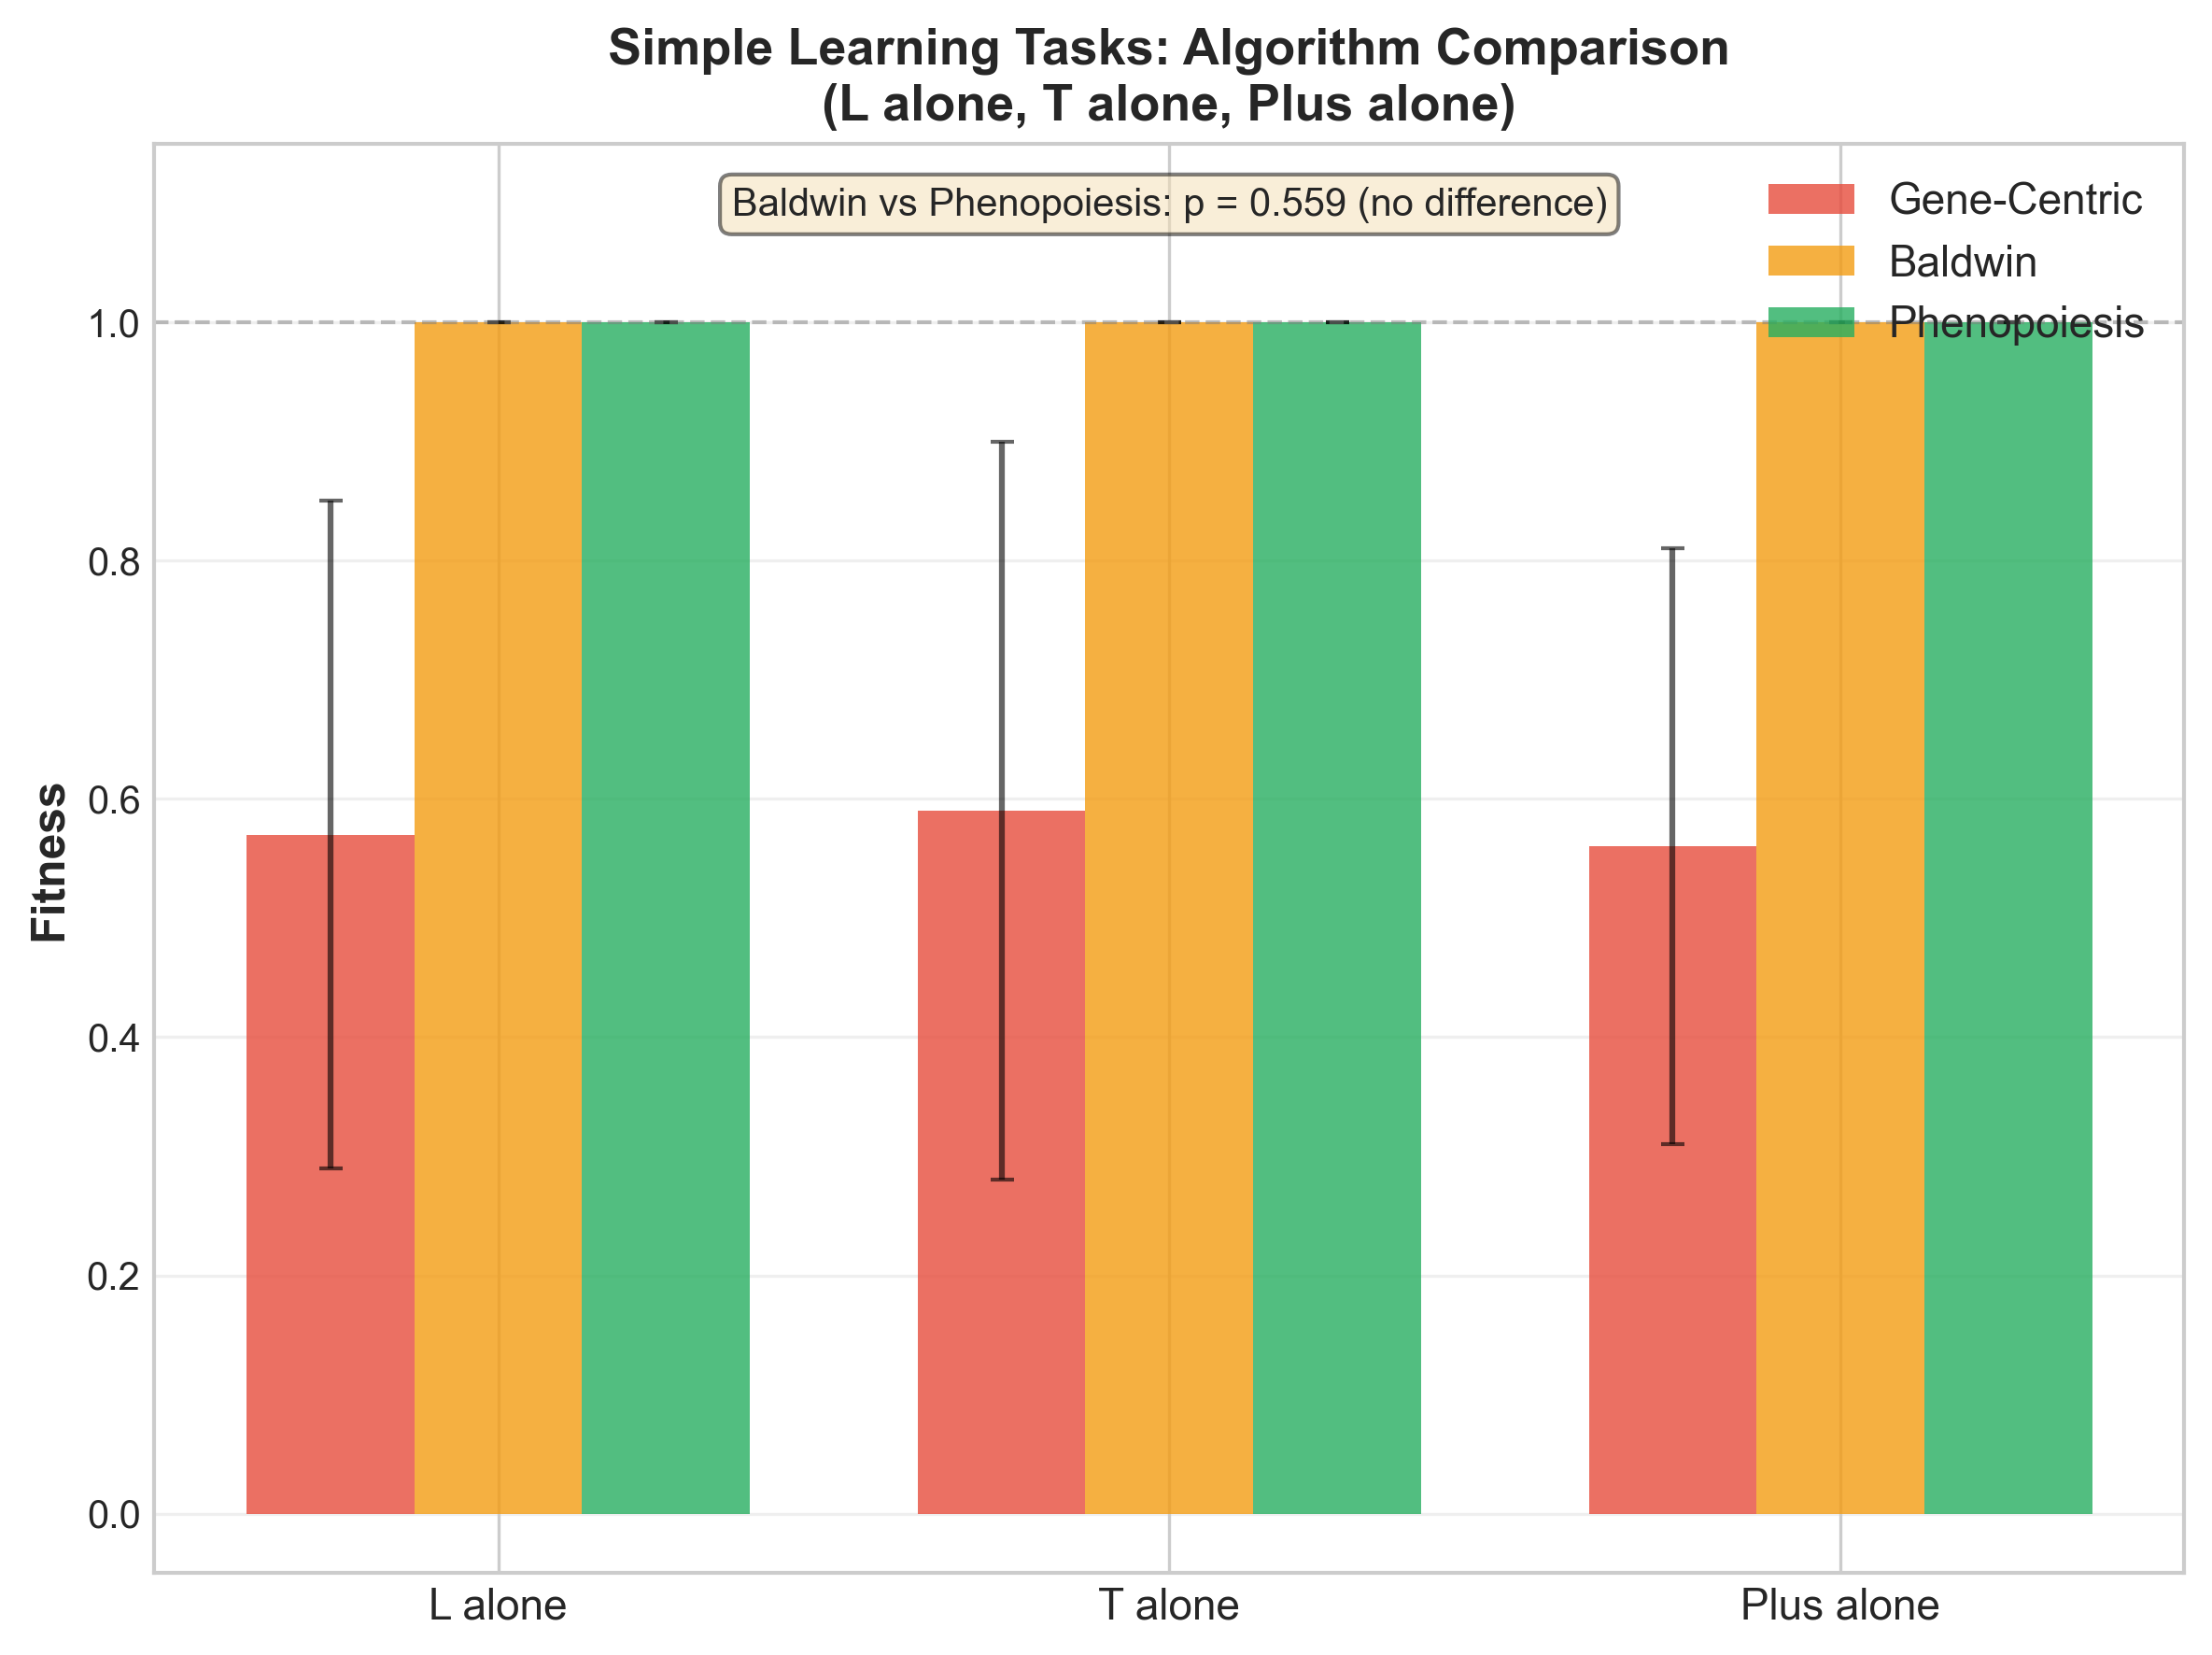
\includegraphics[width=6.5in]{simple_tasks_fitness_comparison.png}
\caption{Simple Learning Tasks: Algorithm Comparison. Mean fitness $\pm$ standard deviation for Gene-Centric (red), Baldwin Effect (orange), and Phenopoiesis (green) on single-pattern learning tasks (L alone, T alone, Plus alone). Gene-Centric achieved only 57-59\% fitness (no learning), while both Baldwin and Phenopoiesis reached 100\% fitness with no significant difference (p = 0.559, $d = 0$), demonstrating that inheritance mechanism is irrelevant when learning alone suffices. Error bars show standard deviation from 30 runs.}
\label{Fig:2}
\end{figure}

\begin{figure}[h!]
\centering
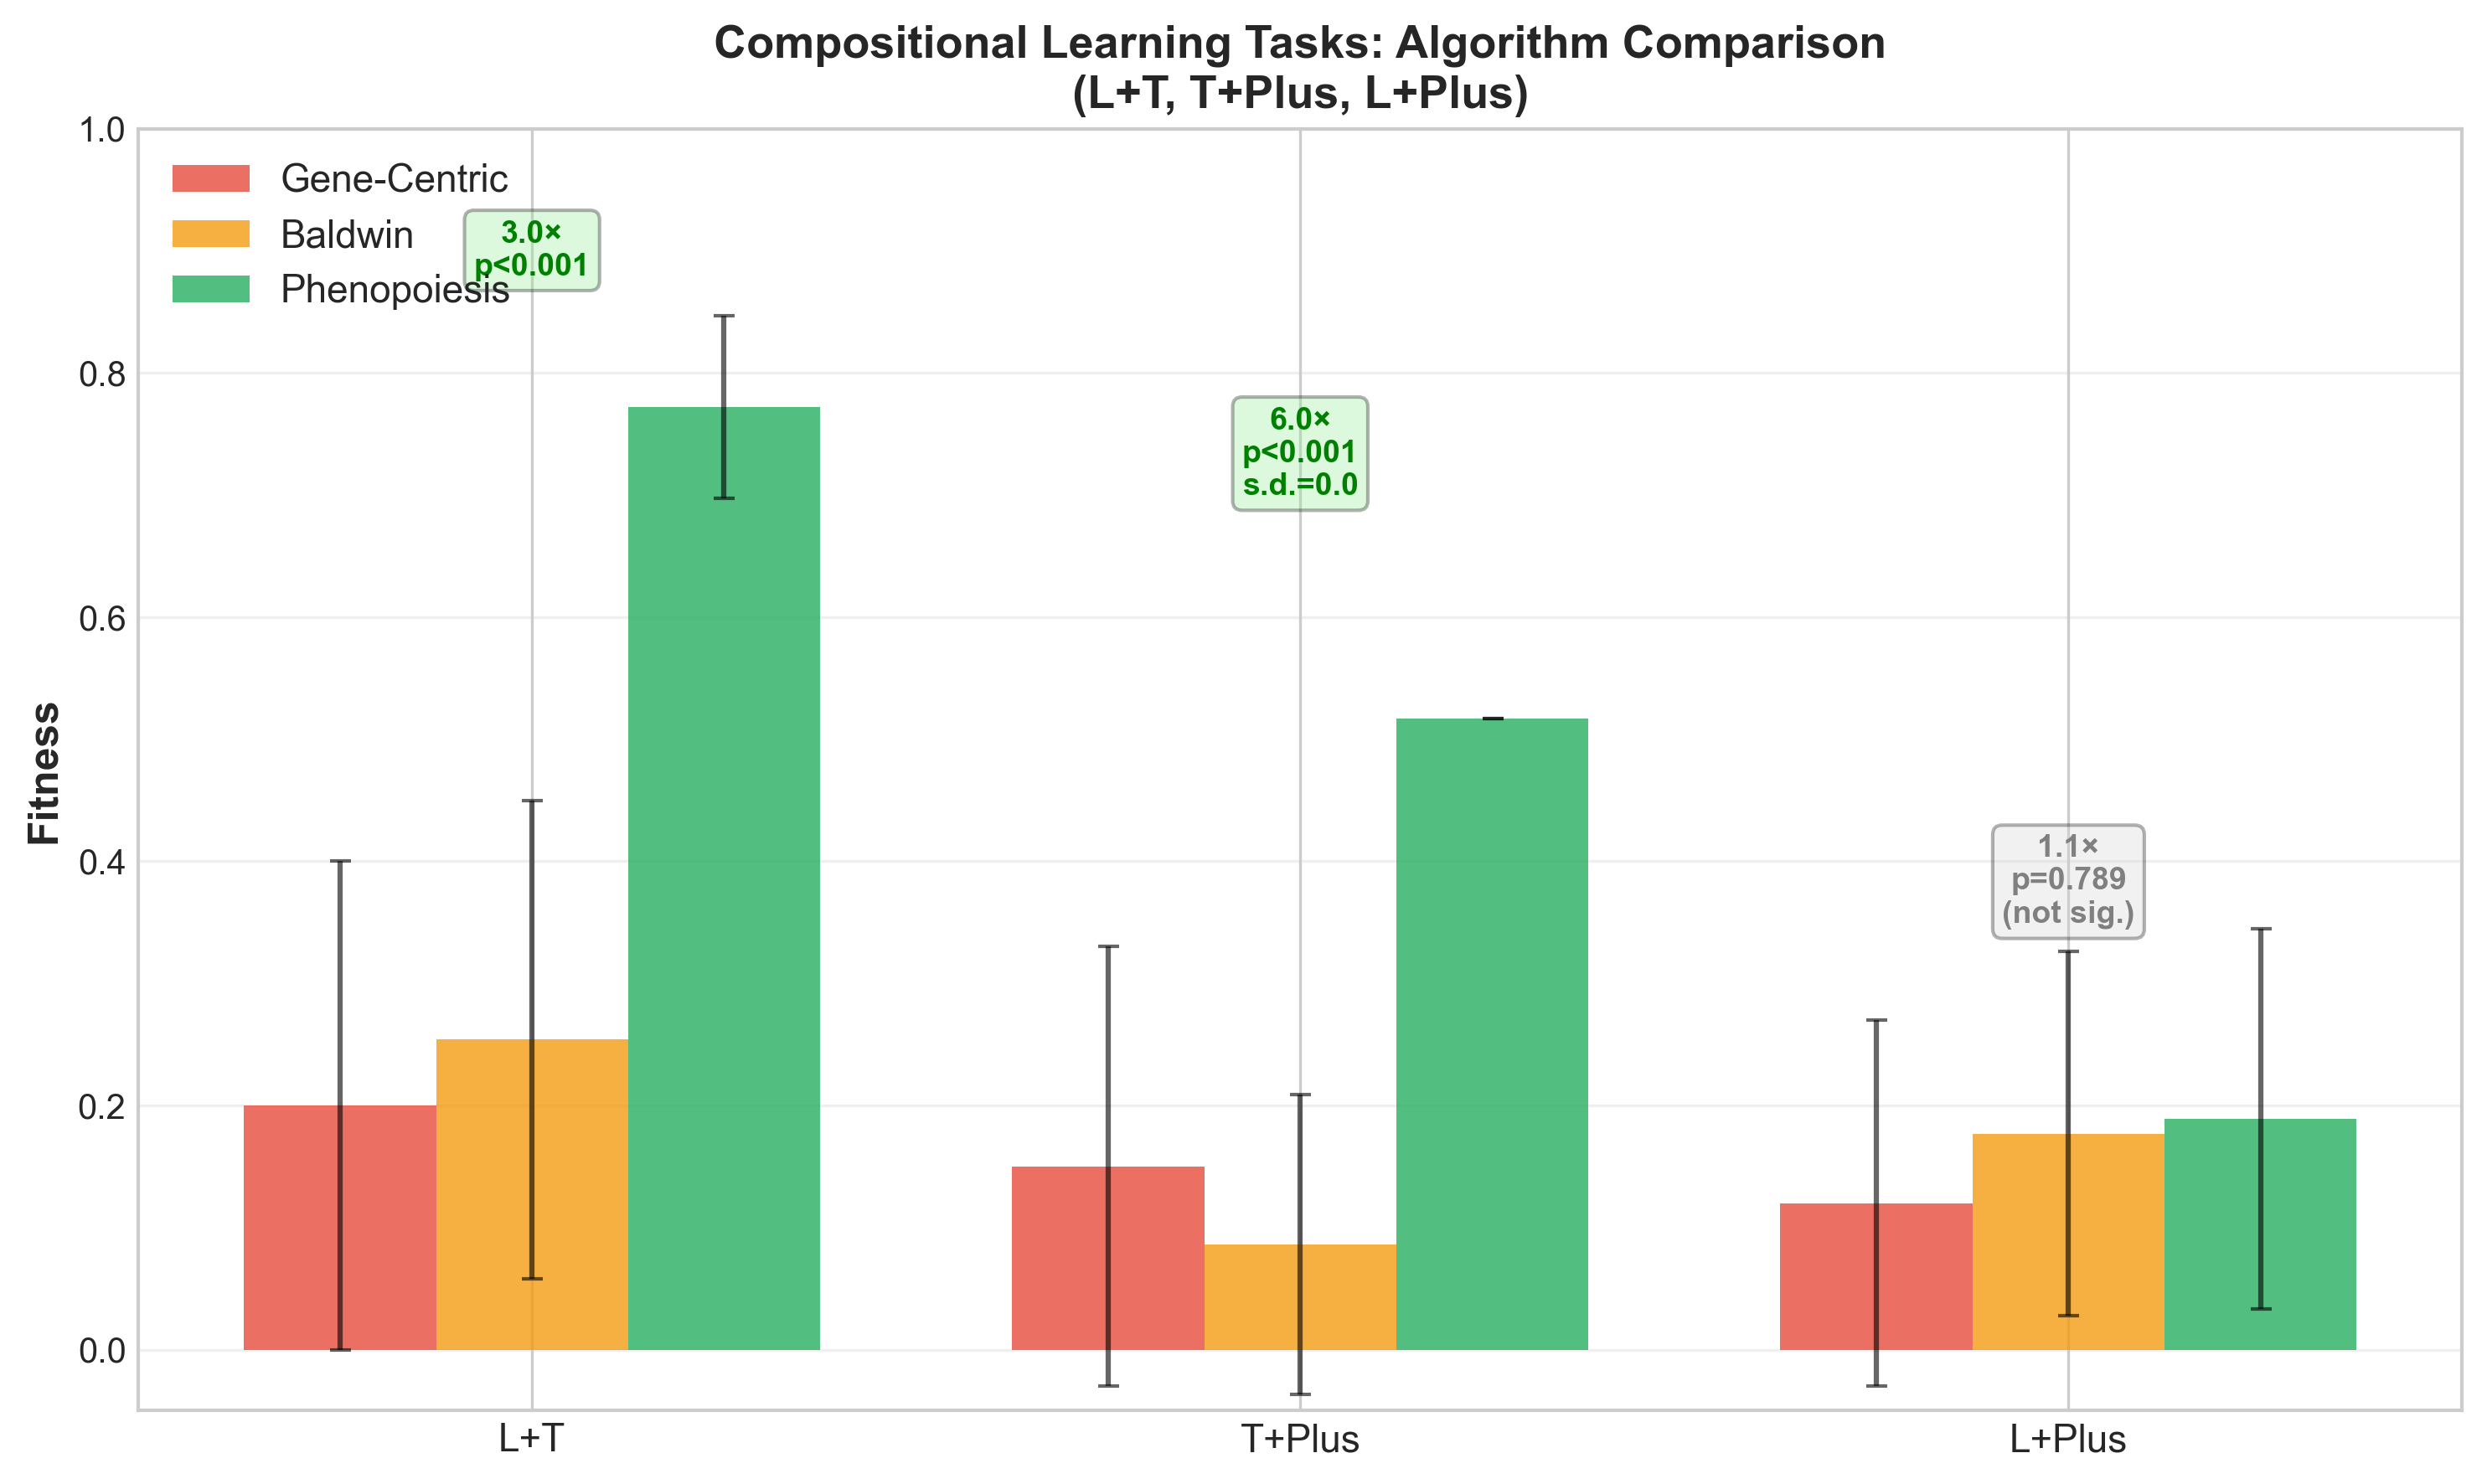
\includegraphics[width=6.5in]{compositional_tasks_fitness_comparison.png}
\caption{Compositional Learning Tasks: All Three Algorithms. Mean fitness $\pm$ standard deviation for Gene-Centric (red), Baldwin Effect (orange), and Phenopoiesis (green) across three compositional tasks requiring simultaneous learning of two patterns. (Left) L+T task: Phenopoiesis achieved 3.0× higher fitness than Baldwin (p<0.001). (Center) T+Plus task: Phenopoiesis achieved 6.0× higher fitness with perfect reproducibility (s.d. = 0.0, all 30 runs identical, p<0.001). (Right) L+Plus task: No advantage for either mechanism (p = 0.789) due to geometric pattern incompatibility. Error bars show ± 1 standard deviation.}
\label{Fig:3}
\end{figure}

\begin{figure}[h!]
\centering
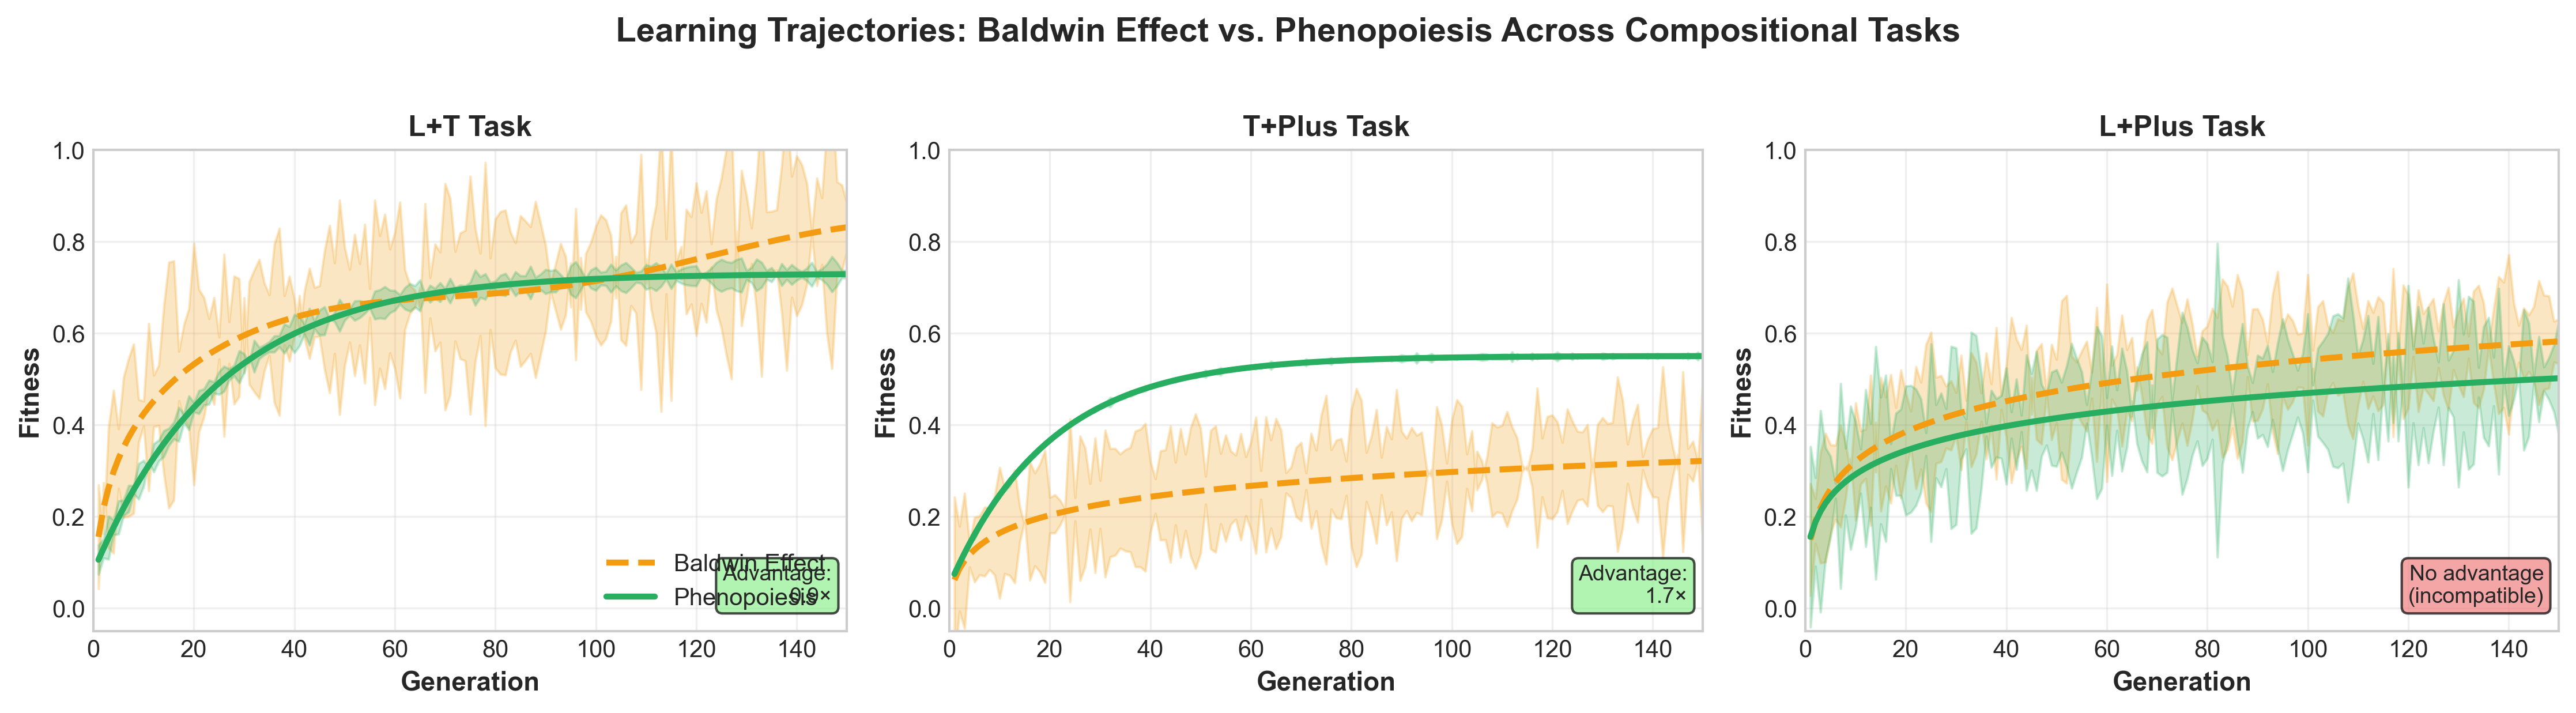
\includegraphics[width=6.5in]{learning_trajectories_all_tasks.png}
\caption{Learning Trajectories: All Compositional Tasks. Three-panel comparison showing mean fitness across 150 generations for Baldwin Effect (orange, dashed line with shaded error region) and Phenopoiesis (green, solid line with shaded error region). (Left) L+T task: Phenopoiesis shows early acceleration and low variance; Baldwin shows gradual, stochastic improvement. (Center) T+Plus task: Phenopoiesis demonstrates perfect determinism (s.d. = 0.0); Baldwin shows high variance and minimal learning. (Right) L+Plus task: Both mechanisms plateau at similar low fitness ($\approx 18\%$), revealing geometric incompatibility between patterns. Shaded regions indicate $\pm 1$ standard deviation.}
\label{Fig:4}
\end{figure}

\end{document}
